\section{Methodology}

\begin{figure*}[t]
    \centering
    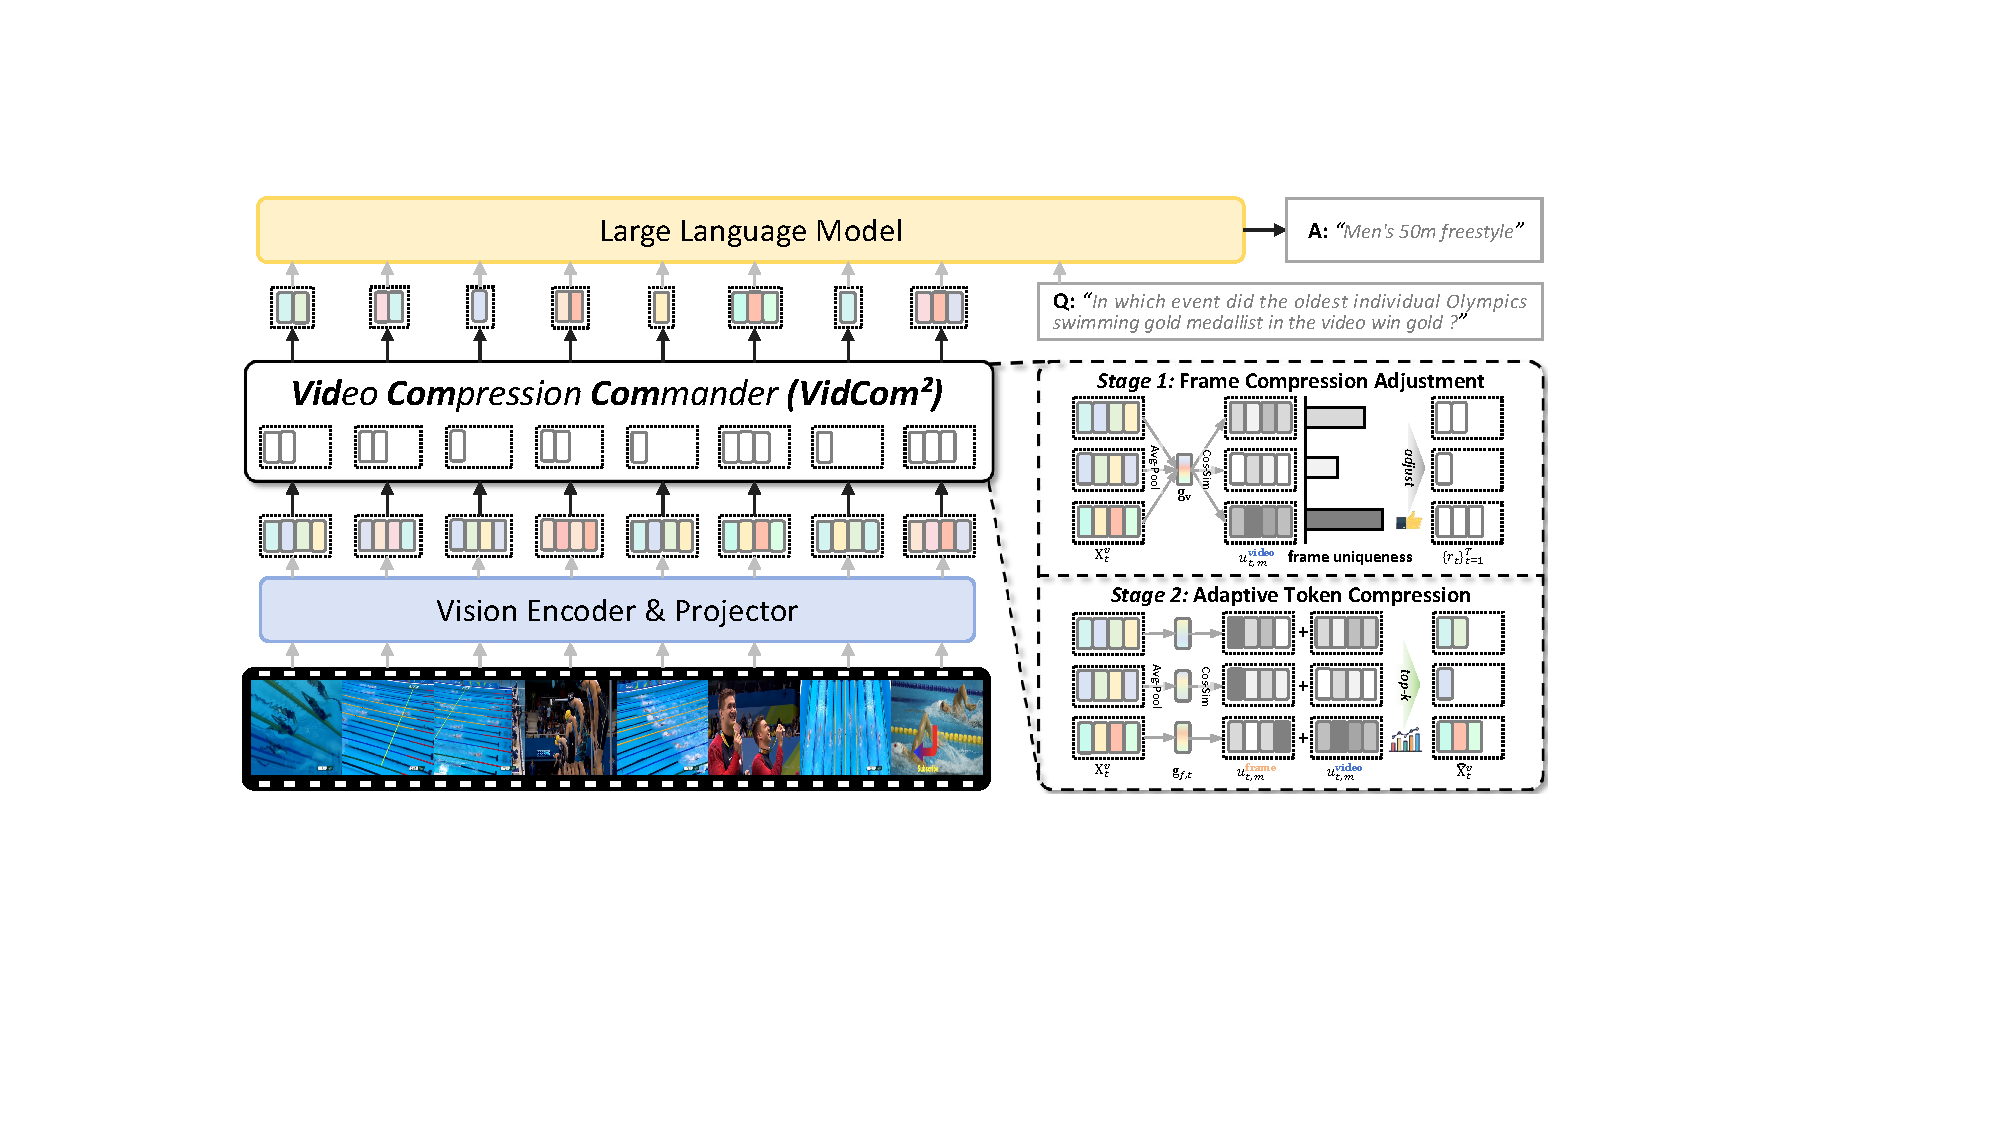
\includegraphics[width=\textwidth]{latex/figures/overview.pdf}
    \vspace{-7mm}
    \caption{\textbf{Overall framework of VidCom$^2$.} Our VidCom$^2$ performs plug-and-play token compression in two stages: \textbf{(i) Frame Compression Adjustment}: adjusts compression intensity based on frame uniqueness (see Figure~\ref{fig:frame_uniqueness_vidcom2}), \textbf{(ii) Adaptive Token Compression}: preserves tokens based on their within-frame and cross-video uniqueness.}
    \vspace{-5mm}
\label{fig:overview}
\end{figure*}


\subsection{Preliminary}

\paragraph{VideoLLM Architecture.} 

Most current VideoLLMs follow the ``ViT-MLP-LLM'' paradigm~\cite{li2024llava-ov,zhang2024llava-video}. For example, in LLaVA-Video, a video sequence $\mathbf{V} = \left\{ \mathbf{v}_t \right\}_{t=1}^T \in \mathbb{R}^{T \times H \times W \times 3}$ is first encoded by ViT into embeddings $\mathbf{Z} = \left\{ \mathbf{z}_t \right\}_{t=1}^T \in \mathbb{R}^{T \times N \times D}$. These embeddings are projected by a 2-layer MLP and pooled to produce visual tokens $\mathbf{X}^v = \left\{ \mathbf{x}_t^v \right\}_{t=1}^T \in \mathbb{R}^{T \times M \times D'}$, with $M < N$, which are then fed into the LLM for autoregressive instruction-following:
{\setlength\abovedisplayskip{2mm}
\setlength\belowdisplayskip{2mm}
\begin{equation}
p\left(\mathbf{Y} \mid \mathbf{X}^{v}, \mathbf{X}^{t}\right)=\prod_{i=1}^L p\left(\mathbf{y}_i \mid \mathbf{X}^{v}, \mathbf{X}^{t}, \mathbf{Y}_{1:i-1}\right),
\end{equation}
}
where $\mathbf{Y}=\left\{ \mathbf{y}_i \right\}_{i=1}^L$ are the generated response tokens, and $\mathbf{X}^{t}$ are the textual tokens.

\paragraph{Token Compression for VideoLLMs.}


Token compression aims to reduce data redundancy by directly compressing token representations for inference acceleration. For VideoLLMs, this typically involves compressing visual token sequences $\mathbf{X}_{t}^v$ into a reduced representation $\mathbf{\hat{X}}^v$:
\begin{equation}
\mathbf{\hat{X}}^v = \boldsymbol{\Phi}(\mathbf{X}^v), \quad \text{where} \quad |\mathbf{\hat{X}}^v| < |\mathbf{X}^v|
\end{equation}
where $\boldsymbol{\Phi}$ represents the token compression operator and $|\cdot|$ denotes the token length.

Token compression is particularly crucial for VideoLLMs due to their processing of substantially more visual tokens compared to standard LVLMs, a result of the multi-frame nature of videos. Consecutive frames often share high similarity, leading to significant visual redundancy. While recent method DyCoke~\cite{tao2024dycoke} address some aspects of multi-frame redundancy, it struggles with uneven frame distinctiveness and achieving aggressive compression rates. Our work focuses on designing an effective token compression operator $\boldsymbol{\Phi}$ that adaptively handles frame-wise distinctiveness while enabling flexible compression rates, addressing these key challenges for VideoLLMs.




\subsection{Video Compression Commander}


To improve the computational efficiency of VideoLLMs, we propose ``\textbf{Vid}eo \textbf{Com}pression \textbf{Com}mander'' (\textbf{VidCom$^2$}), a novel token compression framework that adaptively minimizes visual redundancy within a predefined token budget while preserving distinctive visual information. VidCom$^2$ maintains compatibility with efficient attention operators~\cite{Dao2022:FlashAttention,daoFlashAttention-2} and supports flexible compression rates, enabling plug-and-play inference acceleration.


Figure~\ref{fig:overview} illustrates the overall framework of VidCom$^2$, which achieves efficient token compression for VideoLLMs through a methodical \textbf{\emph{two-stage}} framework: \textbf{(i) Frame Compression Adjustment}, which evaluates frame uniqueness within the video sequence and dynamically allocates optimal token budgets through compression intensity adjustment; and \textbf{(ii) Adaptive Token Compression}, which assesses token distinctiveness both within-frame and across-video, strategically performing compression based on the frame-specific budgets from the previous stage. Below, we elaborate on the detailed operations of these two stages.


\subsection{Stage 1: Frame Compression Adjustment}


The core of this stage is to adaptively adjust compression intensity based on frame uniqueness across the video. A natural question arises: \textbf{\emph{How can a frame's uniqueness be quantified within the video context?}}. Since each frame $\mathbf{x}_t^v \in \mathbb{R}^{M \times D'}$ consists of $M$ visual tokens, we define frame uniqueness through the collective distinctiveness of its constituent tokens.


Specifically, we first obtain a global video representation $\mathbf{g_v}$ by average pooling all tokens across $T$ frames, each with $M$ tokens:
{\setlength\abovedisplayskip{2mm}
\setlength\belowdisplayskip{2mm}
\begin{equation}
\mathbf{g_v} = \frac{1}{T \cdot M} \sum_{t=1}^{T} \sum_{m=1}^{M} \mathbf{x}_{t,m}^v,\quad \mathbf{g_v}\in\mathbb{R}^{D'},
\end{equation}}
where $\mathbf{g_v}$ serves as a coarse-grained summary of the entire video. 
Then, inspired by existing efforts~\cite{sun2025mdp3}, we compute the similarity between each token $\mathbf{x}_{t,m}^v$ and global video representation $\mathbf{g_v}$ in high-dimensional space:
{\setlength\abovedisplayskip{2mm}
\setlength\belowdisplayskip{2mm}
\begin{equation}
s^\mathrm{video}_{t,m} = \frac{\mathbf{x}_{t,m}^v \cdot \mathbf{g_v}}{\|\mathbf{x}_{t,m}^v\|\;\|\mathbf{g_v}\|},\quad s^\mathrm{video}_{t,m}\in[-1,1],
\end{equation}}
where a lower $s^\mathrm{video}_{t,m}$ implies that token $\mathbf{x}_{t,m}^v$ is less redundant (more unique) relative to the full video. We define the \emph{video-level uniqueness score} of token $\mathbf{x}_{t,m}^v$ as $u^\mathrm{video}_{t,m} = -s^\mathrm{video}_{t,m}$ and compute the \emph{frame uniqueness score} $u_t = \frac{1}{M}\sum_{m=1}^{M} u^\mathrm{video}_{t,m}$, where a larger $u_t$ indicates higher density of distinctive tokens in frame $t$ compared to the rest of the video. 
Figure~\ref{fig:frame_uniqueness_vidcom2} demonstrates how $u_t$ effectively quantifies frame-wise uniqueness density within video sequences. More cases are in Appendix~\ref{sec:appendix/more_vis}.



These frame-wise scores $\{u_t\}_{t=1}^T$ are used to modulate per-frame compression intensity. To stabilize the scores, we compute $\tilde{u}_t = (u_t - \max(u_t))/\tau$ ($\tau=0.01$), and obtain the relative importance weight $\sigma_t$ of each frame via softmax:
{\setlength\abovedisplayskip{2mm}
\setlength\belowdisplayskip{2mm}
\begin{equation}
    \sigma_t = \frac{\exp(\tilde{u}_t)}{\sum_{l=1}^{T} \exp(\tilde{u}_l) + \epsilon},
\label{eq:frame_relative_importance}
\end{equation}}
where $\epsilon=10^{-8}$ prevents division by zero. Based on these weights, we adjust the preset retention ratio $R (\%)$ for each frame:
{\setlength\abovedisplayskip{2mm}
\setlength\belowdisplayskip{2mm}
\begin{equation}
    r_t = R \times \left(1 + \sigma_t - \frac{1}{T}\right),
\label{eq:frame_ratio_allocation}
\end{equation}}
where $\sigma_t - \frac{1}{T}$ represents the relative deviation from average importance. Consequently, VidCom$^2$ adaptively adjusts compression intensity (\textit{i.e.}, $\{r_t\}_{t=1}^T$) based on frame uniqueness, enabling differentiated token compression degrees across frames while maintaining the average retention ratio $R$.

\begin{figure*}[!t]
  \centering
   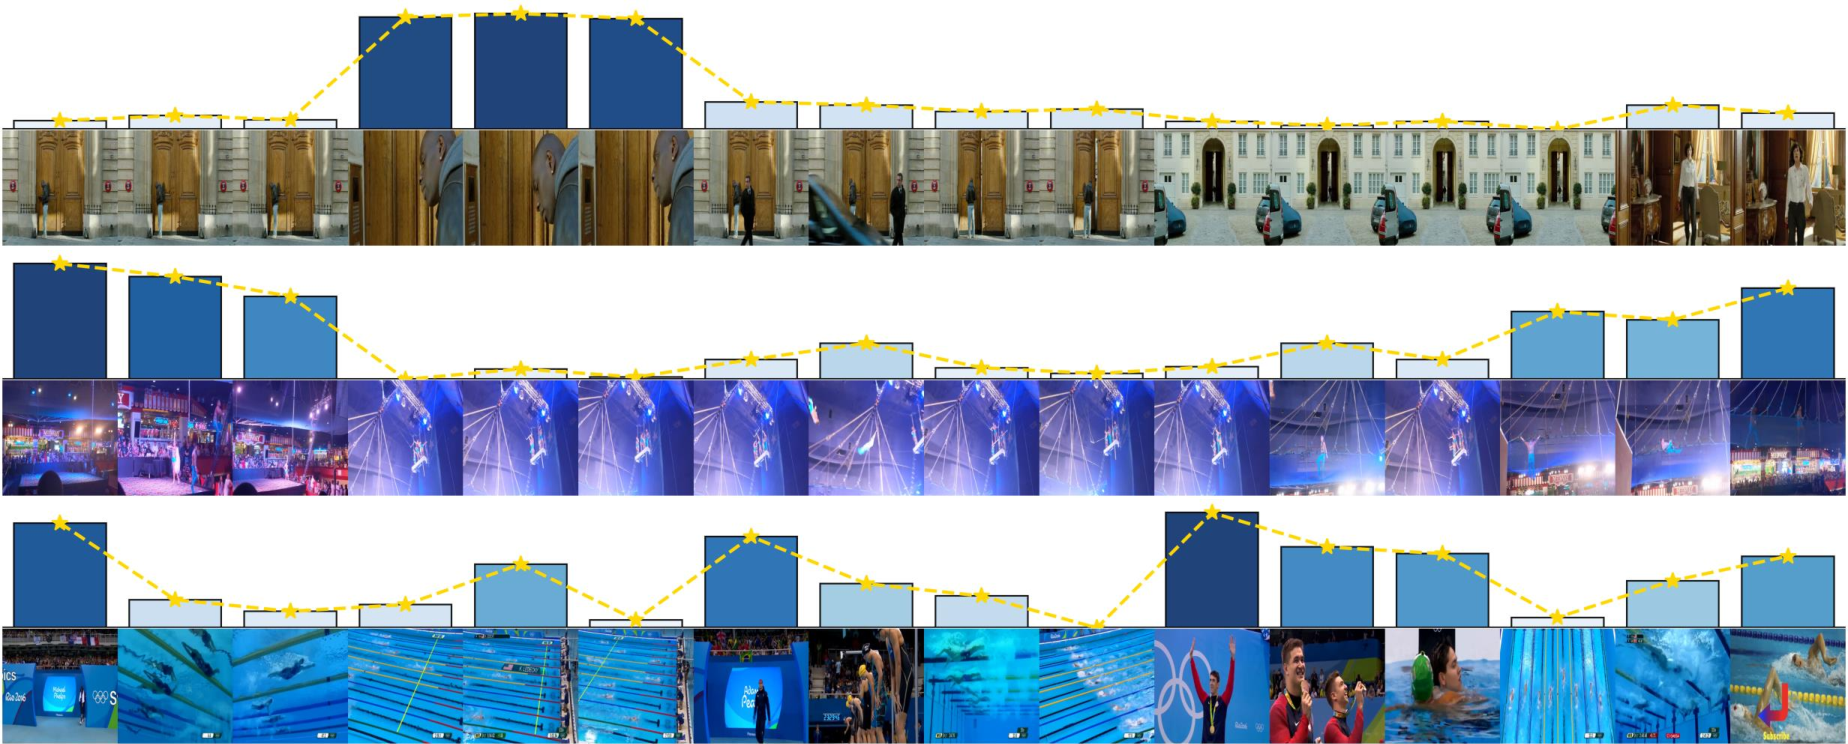
\includegraphics[width=\linewidth]{latex/figures/frame_score_vis.pdf}
   \vspace{-7mm}
    \caption{\textbf{Visualization of frame uniqueness quantified by our VidCom$^2$.} Taller and darker bars indicate frame uniqueness, where VidCom$^2$ allocates more tokens to unique frames to preserve critical visual information.}   
   \label{fig:frame_uniqueness_vidcom2}
   \vspace{-5mm}
\end{figure*}


\subsection{Stage 2: Adaptive Token Compression}


The core of this stage lies in how to select and retain more unique visual information based on the compression degrees $\{r_t\}_{t=1}^T$ determined in the previous stage. Since visual information is composed of tokens, this problem naturally transforms into: \textbf{\emph{How can a token's uniqueness be quantified within the video context?}}. Given the multi-frame nature of videos, a token's uniqueness could be evaluated both locally and globally, \textit{i.e.}, within its frame and across the entire video sequence.


As for token uniqueness within its frame, we can quantify it by measuring its relationship with the frame's global representation. Specifically, for the $t$-th frame, we obtain its global representation through average pooling:
{\setlength\abovedisplayskip{2mm}
\setlength\belowdisplayskip{2mm}
\begin{equation}
\mathbf{g}_{f,t} = \frac{1}{M} \sum_{m=1}^{M} \mathbf{x}_{t,m}^v,\quad \mathbf{g}_{f,t}\in\mathbb{R}^{D'},
\end{equation}}
By computing the cosine similarity of the $m$-th token within the $t$-th frame with its frame-level global representation $\mathbf{g}_{f,t}$, we first define:
{\setlength\abovedisplayskip{2mm}
\setlength\belowdisplayskip{2mm}
\begin{equation}
s^\mathrm{frame}_{t,m} = \frac{\mathbf{x}_{t,m}^v \cdot \mathbf{g}_{f,t}}{\|\mathbf{x}_{t,m}^v\|\;\|\mathbf{g}_{f,t}\|},\quad s_{t,m}\in[-1,1],
\end{equation}}
We then define the \emph{frame-level uniqueness score} as $u^\mathrm{frame}_{t,m} = - s^\mathrm{frame}_{t,m}$, where higher values indicate greater token uniqueness within the frame.



Moreover, since we have already obtained the \emph{video-level uniqueness score} $u^\mathrm{video}_{t,m} = -s^\mathrm{video}_{t,m}$ of token $\mathbf{x}_{t,m}^v$ in the previous stage, we combine these two uniqueness scores to derive \emph{comprehensive uniqueness score} of token $\mathbf{x}_{t,m}^v$ by:
% {\setlength\abovedisplayskip{2mm}
% \setlength\belowdisplayskip{2mm}
% \begin{equation}
% u_{t,m} = \frac{1}{2}\left(u^\mathrm{frame}_{t,m} + u^\mathrm{video}_{t,m}\right),
% \end{equation}}
{\setlength\abovedisplayskip{2mm}
\setlength\belowdisplayskip{2mm}
\begin{equation}
u_{t,m} = u^\mathrm{frame}_{t,m} + u^\mathrm{video}_{t,m},
\end{equation}}
which provides a balanced assessment of the token's distinctiveness both within its frame and across the entire video.

Given the adjusted compression intensity (\textit{i.e.}, $\{r_t\}_{t=1}^T$) based on frame uniqueness in the previous stage, the token compression process for the $t$-th frame can be formulated as:
{\setlength\abovedisplayskip{2mm}
\setlength\belowdisplayskip{2mm}
\begin{equation}
    \mathbf{X}_{t}^{v} \rightarrow \mathbf{\hat{X}}_{t}^{v} = \text{TopK}(\mathbf{X}_{t}^{v}, \{u_{t,m}\}_{m=1}^{M}, r_t \times M)
\end{equation}
}
where $\mathbf{\hat{X}}_{t}^{v}$ represents the compressed token sequence for the $t$-th frame, $\{u_{t,m}\}_{m=1}^{M}$ are the \emph{comprehensive uniqueness scores} of each token in $\mathbf{X}_{t}^{v}$, and $r_t$ is the frame-specific retention ratio. 

To this end, our VidCom$^2$ adaptively adjusts the compression intensity based on frame uniqueness, selectively retaining tokens that are distinctive both within their frames and across the entire video, thereby minimizing information redundancy. The complete algorithm is detailed in Appendix~\ref{sec:appendix/algorithm}.



